% Author: Izaak Neutelings (November, 2018)
% page 8 https://archive.org/details/StaticAndDynamicElectricity
% https://tex.stackexchange.com/questions/56353/extract-x-y-coordinate-of-an-arbitrary-point-on-curve-in-tikz
% https://tex.stackexchange.com/questions/412899/tikz-calculate-and-store-the-euclidian-distance-between-two-coordinates

\documentclass[border=3pt,tikz]{standalone}
\usepackage{amsmath} % for \dfrac
\usepackage{physics,bm}
\usepackage{tikz,pgfplots}
\usepackage[outline]{contour} % glow around text
\usetikzlibrary{angles,quotes} % for pic (angle labels)
\usetikzlibrary{decorations.markings}
\usetikzlibrary{shapes,intersections} % for path name
\tikzset{>=latex} % for LaTeX arrow head
\contourlength{1.4pt}

\usepackage{xcolor}
\colorlet{Ecol}{orange!90!black}
\colorlet{EcolFL}{orange!90!black}
\colorlet{veccol}{green!45!black}
\colorlet{EFcol}{red!60!black}
\tikzstyle{charged}=[top color=blue!20,bottom color=blue!40,shading angle=10]
\tikzstyle{darkcharged}=[very thin,top color=blue!60,bottom color=blue!80,shading angle=10]
\tikzstyle{charge+}=[very thin,top color=red!80,bottom color=red!80!black,shading angle=-5]
\tikzstyle{charge-}=[very thin,top color=blue!50,bottom color=blue!70!white!90!black,shading angle=10]
\tikzstyle{darkcharged}=[very thin,top color=blue!60,bottom color=blue!80,shading angle=10]
\tikzstyle{gauss surf}=[green!70!black,top color=green!2,bottom color=green!80!black!70,shading angle=5,fill opacity=0.6]
\tikzstyle{gauss lid}=[gauss surf,middle color=green!80!black!20,shading angle=40,fill opacity=0.7]
\tikzstyle{gauss dark}=[green!60!black,fill=green!60!black!70,fill opacity=0.8]
\tikzstyle{gauss line}=[green!80!black]
\tikzstyle{gauss dashed line}=[green!60!black!80,dashed,line width=0.2]
\tikzstyle{vector}=[->,thick,veccol]
\tikzstyle{normalvec}=[->,thick,blue!80!black!80]
\tikzstyle{EField}=[->,thick,Ecol]
\tikzstyle{EField dashed}=[dashed,Ecol,line width=0.6]
\tikzset{
  EFieldLine/.style={thick,EcolFL,decoration={markings,
                     mark=at position #1 with {\arrow{latex}}},
                     postaction={decorate}},
  EFieldLine/.default=0.5}
\tikzstyle{measure}=[fill=white,midway,outer sep=2]
\def\L{2.2}
\def\H{2.2}
\def\offset{2.0}
\def\W{0.30}
\def\Nx{5}
\def\Ny{5}


\begin{document}


% PLANE charge distribution
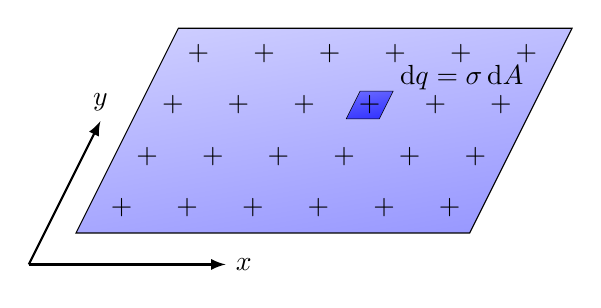
\begin{tikzpicture}[x={(1,0)},y={(0.5,1)}]%,z={(0.73cm,0.73cm)}
  \def\H{2.6}
  \def\W{5.0}
  \def\Nx{6}
  \def\Ny{4}
  \def\h{0.35}
  \def\w{0.42}
  \coordinate (P) at (3.5*\W/\Nx,2.5*\H/\Ny);
  
  % AXES
  \begin{scope}[shift={(-0.08*\W,-0.08*\W)}]
    \draw[->,thick] (0,0) -- (0,0.7*\H) node[above] {$y$};
    \draw[->,thick] (0,0) -- (0.5*\W,0) node[right] {$x$};
  \end{scope}
  
  % PLANE
  \draw[charged]
    (0,0) --++ (\W,0) --++ (0,\H) --++ (-\W,0) -- cycle;
  \foreach \i [evaluate={\x=(\i-0.5)*\W/\Nx;}] in {1,...,\Nx}{
    \foreach \j [evaluate={\y=(\j-0.5)*\H/\Ny;}] in {1,...,\Ny}{
      \node[scale=1.0,rotate=0] at (\x,\y) {$+$};
    }
  }
  
  % CHARGE
  \draw[darkcharged]
    (P) ++ (-\w/2,-\h/2) --++ (\w,0) --++ (0,\h) coordinate (C) --++ (-\w,0) -- cycle;
  \node[above=5,right=-1,scale=1.0] at (C) {$\dd{q}=\sigma \dd{A}$};
  \node[scale=1.0] at (P) {$+$};
  
\end{tikzpicture}


% ROUND RING integration
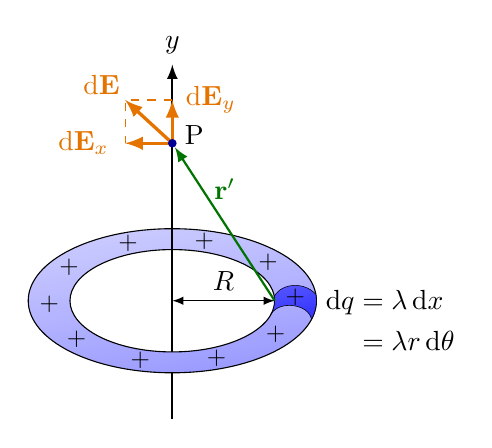
\begin{tikzpicture}[x={(1,0)},y={(0,0.5)}]
  \def\r{1.3}
  \def\dr{0.53}
  \def\dtu{5}   % upper angle dq segment
  \def\dtd{-15} % lower angle dq segment
  \def\Ex{0.6}
  \def\Ey{1.1}
  \def\N{10}
  \coordinate (O) at (0,0);
  \coordinate (P) at (0,4.0);
  \coordinate (Y) at (0,6.0);
  \coordinate (-Y) at (0,-3.0);
  \coordinate (R) at (\r,0);
  
  % PLANE
  \draw[thick] (O) -- (-Y); % axis below
  \draw[charged,even odd rule]
    (O) circle (\r+\dr) circle (\r);
  \draw[darkcharged]
    (O) ++ (\dtu:\r) arc (\dtu:\dtd:\r) to[out=60,in=100]++ (\dtd:\dr) arc (\dtd:\dtu:\r+\dr) to[out=130,in=60] cycle;
  \foreach \i [evaluate={\cang=3+\i*360/\N;}] in {1,...,\N}{
    \node[scale=0.9,rotate=0] at (\cang:\r+\dr/2) {$+$};
  }
  
  % CHARGE
  %\node[below=1,right=0,scale=1.0] at (4:\r+\dr) {$\dd{q} = \lambda \dd{x} = \lambda r\dd{\theta}$};
  \node[below=10,right=0,scale=1.0] at (4:\r+\dr) {
    $\begin{aligned}
       \dd{q} &= \lambda \dd{x}\\
              &= \lambda r\dd{\theta}
    \end{aligned}$
  };
  
  % AXIS
  \draw[->,thick] (O) -- (Y) node[above] {$y$};
  
  % VECTORS
  \draw[EField,very thick] (P) --++ ( 0.0,\Ey) node[right=1] {$\dd{\vb{E}_y}$};
  \draw[EField,very thick] (P) --++ (-\Ex,0.0) node[left=2] {$\dd{\vb{E}_x}$};
  \draw[EField,very thick] (P) --++ (-\Ex,\Ey) node[above left=-2] {$\dd{\vb{E}}$};
  \draw[EField,-,dashed,thin] (P) ++ (0,\Ey) --++ (-\Ex,0) --++ (0,-\Ey);
  \node[fill=blue!60!black,circle,inner sep=1.1] (P') at (P) { };
  \node[above=3,right=1] at (P') {P};
  \draw[vector,veccol] (R) -- (P') node[midway,above=5] {$\vb{r}'$};
  \draw[<->] (0,0) --++ (0:\r) node[midway,above] {$R$};
  
\end{tikzpicture}


% ROUND SHEET integration
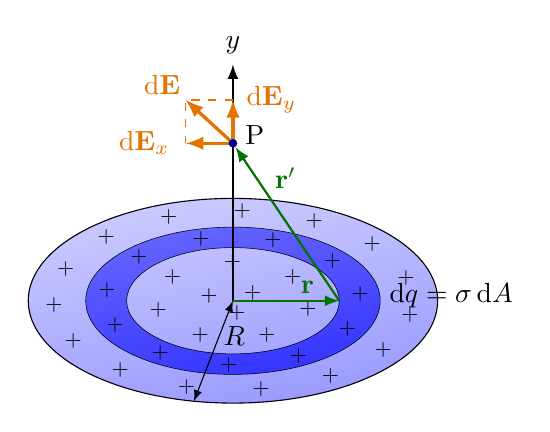
\begin{tikzpicture}[x={(1,0)},y={(0,0.5)}]
  \def\R{2.6}
  \def\r{1.35}
  \def\dr{0.52}
  \def\Ex{0.6}
  \def\Ey{1.1}
  \def\Nx{4}
  \coordinate (O) at (0,0);
  \coordinate (P) at (0,4.0);
  \coordinate (Y) at (0,6.0);
  \coordinate (R) at (\r,0);
  
  % PLANE
  \draw[charged]
    (O) circle (\R);
  \draw[darkcharged,even odd rule]
    (O) circle (\r+\dr) circle (\r);
  \foreach \i [evaluate={\cr=(\i-0.5)*\R/\Nx; \Ny=7+4*(\i-2);}] in {1,...,\Nx}{
    \foreach \j [evaluate={\cang=39+\j*360/\Ny;}] in {1,...,\Ny}{
      \node[scale=0.8,rotate=0] at (\cang:\cr) {$+$};
    }
  }
  
  % CHARGE
  \node[right=0,scale=1.0] at (4:\r+\dr) {$\dd{q}=\sigma \dd{A}$};
  
  % AXIS
  \draw[->,thick] (0,0) -- (Y) node[above] {$y$};
  
  % VECTORS
  \draw[EField,very thick] (P) --++ ( 0.0,\Ey) node[right=1] {$\dd{\vb{E}_y}$};
  \draw[EField,very thick] (P) --++ (-\Ex,0.0) node[left=2] {$\dd{\vb{E}_x}$};
  \draw[EField,very thick] (P) --++ (-\Ex,\Ey) node[above left=-2] {$\dd{\vb{E}}$};
  \draw[EField,-,dashed,thin] (P) ++ (0,\Ey) --++ (-\Ex,0) --++ (0,-\Ey);
  \node[fill=blue!60!black,circle,inner sep=1.1] (P') at (P) { };
  \node[above=3,right=1] at (P') {P};
  \draw[vector,veccol] (R) -- (P') node[pos=0.8,right=3] {$\vb{r}'$};
  \draw[vector,veccol] (0,0) --++ (0:\r) node[pos=0.7,above=-1] {$\vb{r}$};
  \draw[<->] (0,0) --++ (-101:\R) node[pos=0.35,right=-2] {$R$};
  
\end{tikzpicture}


% PLANE field with electric field
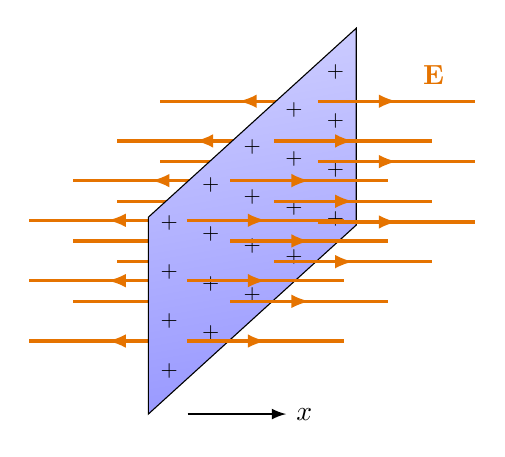
\begin{tikzpicture}[x={(1.0cm,0)},y={(0.55cm,0.5cm)},z={(0,1.0cm)}]
  \def\H{2.5}
  \def\W{4.8}
  \def\Ny{5}
  \def\Nz{4}
  \def\NEy{4}
  \def\NEz{3}
  \def\oEy{0.08*\W}
  \def\oEz{0.04*\H}
  \def\E{2}
  \coordinate (O) at (0.0,-0.5,-0.5);
  
  % AXES
  \draw[->,thick] (0.5,0,0) --++ (0.5*\H,0,0) node[right] {$x$};
  %\draw[->,thick] (O) --++ (0.5*\H,0,0) node[right] {$x$};
  %\draw[->,thick] (O) --++ (0,0.7*\H,0) node[right] {$y$};
  %\draw[->,thick] (O) --++ (0,0,0.5*\H) node[above] {$z$};
  
  % ELECTRIC FIELD back
  \foreach \i [evaluate={\y=\oEy+(\i-0.5)*(\W-2*\oEy)/\NEy;}] in {1,...,\NEy}{
    \foreach \j [evaluate={\z=\oEz+(\j-0.5)*(\H-2*\oEz)/\NEz;}] in {1,...,\NEz}{
      \draw[EFieldLine,very thick] (0,\y,\z) --++ (-\E,0,0);
    }
  }
  
  % PLANE
  \draw[charged]
    (0,0,0) --++ (0,\W,0) --++ (0,0,\H) --++ (0,-\W,0) -- cycle;
  \foreach \i [evaluate={\y=(\i-0.5)*\W/\Ny;}] in {1,...,\Ny}{
    \foreach \j [evaluate={\z=(\j-0.5)*\H/\Nz;}] in {1,...,\Nz}{
      \node[scale=0.8,rotate=0] at (0,\y,\z) {$+$};
    }
  }
  
  % ELECTRIC FIELD front
  \foreach \i [evaluate={\y=\oEy+(\i-0.5)*(\W-2*\oEy)/\NEy;}] in {1,...,\NEy}{
    \foreach \j [evaluate={\z=\oEz+(\j-0.5)*(\H-2*\oEz)/\NEz;}] in {1,...,\NEz}{
      \draw[EFieldLine,very thick] (0,\y,\z) --++ (\E,0,0);
    }
  }
  \node[Ecol] at (1.3,0.88*\W,0.88*\H) {$\vb{E}$};
  
  
\end{tikzpicture}


% PLANE field with gaussian surface
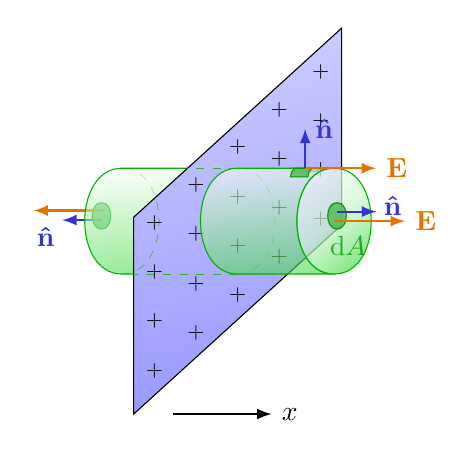
\begin{tikzpicture}[x={(1.0cm,0)},y={(0.55cm,0.5cm)},z={(0,1.0cm)}]
  \def\H{2.5}
  \def\W{4.8}
  \def\Ny{5}
  \def\Nz{4}
  \def\R{0.14*\W}
  \def\a{0.49*\H}
  \def\E{0.36*\H}
  \def\plane{(0,0,0) --++ (0,\W,0) --++ (0,0,\H) --++ (0,-\W,0) -- cycle;}
  \coordinate (O) at (0.0,-0.5,-0.5);
  \coordinate (C)  at (      0,\W/2,\H/2);
  \coordinate (ER) at (     \a,\W/2,\H/2);
  \coordinate (EL) at (-1.2*\a,\W/2-0.6*\R,\H/2+0.5*\R);
  \coordinate (TM) at (      0,\W/2,\H/2+\R);
  \coordinate (TR) at (     \a,\W/2,\H/2+\R);
  \coordinate (TL) at (-1.2*\a,\W/2,\H/2+\R);
  \coordinate (BM) at (      0,\W/2,\H/2-\R);
  \coordinate (BR) at (     \a,\W/2,\H/2-\R);
  \coordinate (BL) at (-1.2*\a,\W/2,\H/2-\R);
  \coordinate (NT) at (0.7*\a,\W/2,\H/2+\R);
  \coordinate (NR) at (\a,\W/2+0.13*\R,\H/2+0.13*\R);
  \coordinate (NL) at (-1.2*\a,\W/2-0.5*\R,\H/2-0.2*\R);
  \coordinate (NB) at (0.86*\a,\W/2-0.6*\R,\H/2-0.6*\R);
  
  % AXES
  \draw[->,thick] (0.5,0,0) --++ (0.5*\H,0,0) node[right] {$x$};
  
  % VECTORS back
  \draw[EField] (EL) --++ (-\E,0,0);
  \draw[normalvec] (EL) ++(0,-0.1*\R,-0.13*\R) --++ (-0.5,0,0) node[below left=-1] {$\vu{n}$};
  \draw[gauss dark]
    (EL)++(0,-0.1*\R,-0.3*\R)
      to[out=0,in=0,looseness=1.2] ++(0,0,0.5*\R)
      to[out=180,in=180,looseness=1.2] ++(0,0,-0.5*\R) -- cycle; %node[left=4,below=-1] {$\dd{A}$};
  
  % GAUSSIAN SURFACE back
  \draw[gauss dashed line] (BL) to[out=0,in=0,looseness=1.2] (TL);
  \draw[gauss surf]
    (BM) to[out=180,in=180,looseness=1.2] (TM) --
    (TL) to[out=180,in=180,looseness=1.2] (BL) -- cycle;
  
  % PLANE
  \draw[charged] \plane;
  \begin{scope}
    \clip \plane;
    \draw[gauss dashed line] (BM) -- (BL);
    \draw[gauss dashed line] (TM) -- (TL);
    \draw[gauss dashed line] (BL) to[out=0,in=0,looseness=1.2] (TL);
  \end{scope}
  \foreach \i [evaluate={\y=(\i-0.5)*\W/\Ny;}] in {1,...,\Ny}{
    \foreach \j [evaluate={\z=(\j-0.5)*\H/\Nz;}] in {1,...,\Nz}{
      \node[scale=0.8,rotate=0] at (0,\y,\z) {$+$};
    }
  }
  \draw[gauss dark]
    (NT) ++ (-0.12,0,0) to[out=-5,in=110] ++(0,0.12,-0.10) --++(0.22,0,0) to[out=110,in=-5] ++(0,-0.12,0.10) -- cycle;
  
  % GAUSSIAN SURFACE front
  \draw[gauss dashed line]
    (BM) to[out=0,in=0,looseness=1.2] (TM);
  \draw[gauss surf]
    (BM) to[out=180,in=180,looseness=1.2] (TM) --
    (TR) to[out=180,in=180,looseness=1.2] (BR) -- cycle;
  \draw[gauss lid]
    (BR) to[out=0,in=0,looseness=1.2] (TR) to[out=180,in=180,looseness=1.2] cycle;
  
  % DARK
  \draw[gauss dark]
    (NT) ++ (-0.12,0,0) to[out=-160,in=80] ++(0,-0.12,-0.05) --++(0.22,0,0) to[out=80,in=-160] ++(0,0.12,0.05) -- cycle;
  \draw[gauss dark]
    (ER)++(0,0.1*\R,-0.2*\R)
      to[out=0,in=0,looseness=1.2] ++(0,0,0.5*\R)
      to[out=180,in=180,looseness=1.2] ++(0,0,-0.5*\R) -- cycle node[right=4,below=-1] {$\dd{A}$};
  
  % ELECTRIC FIELD
  \draw[EField] (ER) --++ (\E,0,0) node[right] {$\vb{E}$};
  \draw[EField] (NT) --++ (\E,0,0) node[right] {$\vb{E}$};
  
  % VECTORS
  \draw[normalvec] (ER) ++(0,0.1*\R,0.13*\R) --++ (0.5,0,0) node[above=2,right=-1] {$\vu{n}$};
  \draw[normalvec] (NT) --++ (0,0,0.5) node[right] {$\vu{n}$};
  %\draw[normalvec] (NB) --++ (0,-0.35,-0.25) node[below right=-2] {$\vu{n}$};
  
  
\end{tikzpicture}




% GAUSSIAN
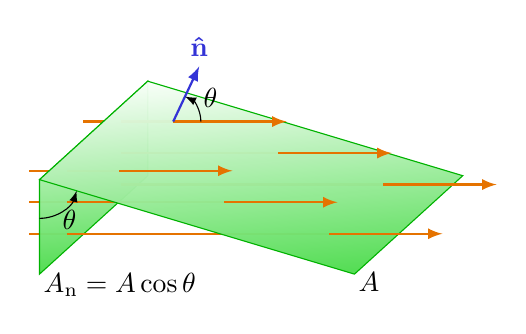
\begin{tikzpicture}[x={(1.0cm,0)},y={(0.55cm,0.5cm)},z={(0,1.0cm)}]
  \def\H{1.2}
  \def\W{2.5}
  \def\L{4.0}
  \def\Ny{2}
  \def\Nz{3}
  \def\ER{0.4*\H}
  \def\E{1.2*\H}
  \coordinate (O) at (0,0,0);
  \coordinate (T) at (0,0,\H);
  \coordinate (R) at (\L,0,0);
  
  % COORDINATES
  \message{Coordinates}
  \foreach \j [evaluate={\z=(\j-0.5)*\H/\Nz; \x=(\H-\z)*\L/\H;}] in {1,...,\Nz}{
    \foreach \i [evaluate={\y=(\i-0.5)*\W/\Ny};] in {1,...,\Ny}{
      \message{ (\i,\j) -> (\x,\y,\z)^^J}
      \coordinate (EL\i\j) at (0,\y,\z);
      \coordinate (ER\i\j) at (\x,\y,\z);
    }
  }
  
  % ELECTRIC FIELDS back
  \draw[EField,-] (EL11) --++ (-\ER,0,0);
  \draw[EField,-] (EL12) --++ (-\ER,0,0);
  \draw[EField,-] (EL13) --++ (-\ER,0,0);
  \draw[EField,-] (EL21) --++ (-\ER,0,0);
  \draw[EField,-] (EL22) --++ (-\ER,0,0);
  \draw[EField,-] (EL23) --++ (-\ER,0,0);
  
  % PLANE
  \draw[gauss surf,fill opacity=0.97] (O) --++ (0,\W,0) --++ (0,0,\H) --++ (0,-\W,0) -- cycle;
  
%  % ELECTRIC FIELDS middle
%  \begin{scope}
%    \clip (O) -- (T) -- (R) -- cycle;
%    \draw[EField dashed] (EL11) --++ (-\ER,0,0);
%    \draw[EField dashed] (EL12) --++ (-\ER,0,0);
%    \draw[EField dashed] (EL13) --++ (-\ER,0,0);
%    \draw[EField dashed] (EL21) --++ (-\ER,0,0);
%    \draw[EField dashed] (EL22) --++ (-\ER,0,0);
%    \draw[EField dashed] (EL23) --++ (-\ER,0,0);
%  \end{scope}
  
  % ELECTRIC FIELDS
  \draw[EField,-] (EL11) -- (ER11);
  \draw[EField,-] (EL12) -- (ER12);
  \draw[EField,-] (EL13) -- (ER13);
  \draw[EField,-] (EL21) -- (ER21);
  \draw[EField,-] (EL22) -- (ER22);
  \draw[EField,-] (EL23) -- (ER23);
  
  % PLANE
  \draw[gauss surf,name path=skew,fill opacity=0.97]
    (0,0,\H) --++ (0,\W,0) --++ (\L,0,-\H) --++ (0,-\W,0) -- cycle;
  
  % ELECTRIC FIELDS
  \draw[EField] (ER11) --++ (\E,0,0);
  \draw[EField] (ER12) --++ (\E,0,0);
  \draw[EField] (ER13) --++ (\E,0,0);
  \draw[EField] (ER21) --++ (\E,0,0);
  \draw[EField] (ER22) --++ (\E,0,0);
  \draw[EField] (ER23) --++ (\E,0,0) coordinate (ET);
  
  % VECTORS
  \draw[normalvec] (ER23) --++ (0.33,0,0.7) node[above] {$\vu{n}$} coordinate (N);
  
  % ANGLES
  \draw pic[->,"$\theta$",draw=black,angle radius=14,angle eccentricity=1.3] {angle = O--T--R};
  \draw pic[->,"$\theta$",draw=black,angle radius=10,angle eccentricity=1.6] {angle = ET--ER23--N};
  
  % LABELS
  \node[above=2,below right=-2] at (O) {$A_\mathrm{n} = A\cos\theta$};
  \node[above=2,below right=-2] at (R) {$A$};
  
\end{tikzpicture}




\end{document}
